\documentclass[a4paper, 12pt]{report}
\usepackage[T1]{fontenc}
\usepackage{geometry}
\usepackage[normalem]{ulem}
\geometry{verbose,a4paper,tmargin=1in,bmargin=1in,lmargin=1.5in,rmargin=1in}
\usepackage{graphicx}
\usepackage{setspace}
\setstretch{1.8}
\usepackage{seqsplit}
\usepackage{ltxtable}
\usepackage{array,longtable}
\usepackage{hyphenat}
\usepackage{algorithmic}
\usepackage{algorithm}
\usepackage{relsize}
\usepackage{amsmath}
\usepackage{varwidth}
\usepackage{subfig}
\usepackage{nicefrac}
\usepackage{fixltx2e}
\usepackage{amsfonts}
\usepackage{float}
\usepackage{multirow}
\usepackage{cellspace}
\usepackage{morefloats}
\usepackage{amssymb}
\usepackage{cite}
\DeclareGraphicsExtensions{.eps}
\usepackage{nomencl}
\usepackage{import}
\makenomenclature
\usepackage[nottoc,numbib]{tocbibind}
\usepackage{amsmath}
\usepackage{fancyhdr}
\setcounter{secnumdepth}{5}
\setcounter{tocdepth}{5}
\onehalfspacing
\usepackage[colorlinks=true, linkcolor=black, citecolor=black, urlcolor=black]{hyperref} % for hyperlinks in the document
\usepackage{listings}
\usepackage{color}
\definecolor{gb}{rgb}{0,0.5,0.5}
\definecolor{red}{rgb}{0.5,0,0}
\lstset{
    keywordstyle=\small\bf\color{blue},
    commentstyle=\small\color{gb},
    stringstyle=\small\color{red},
}

% Customizing Chapter and Section Title Formats
\usepackage{titlesec}
\titleformat{\chapter}[display]
  {\normalfont\huge\bfseries}{Chapter \thechapter}{20pt}{\Huge}
\titleformat{\section}
  {\normalfont\large\bfseries}{\thesection}{1em}{}
  
  












\usepackage{indentfirst}
\usepackage{enumitem}

\usepackage{multicol} % Package for multiple columns
\usepackage{courier} % Use Courier font for code
\usepackage{fontenc} % Load this package if needed for specific font encodings
\usepackage{xcolor} % For coloring
\usepackage{tcolorbox} % For the terminal box
\tcbuselibrary{listingsutf8, skins} % Load the necessary tcolorbox libraries

\setlength{\parindent}{0pt}
\definecolor{myblue}{RGB}{0,0,128}


% Code style
\definecolor{codegreen}{rgb}{0,0.6,0}
\definecolor{codegray}{rgb}{0.5,0.5,0.5}
\definecolor{codepurple}{rgb}{0.58,0,0.82}
\definecolor{backcolour}{rgb}{0.95,0.95,0.92}
\lstdefinestyle{mystyle}{
    backgroundcolor=\color{backcolour},
    commentstyle=\color{codegreen},
    keywordstyle=\color{magenta},
    numberstyle=\tiny\color{codegray},
    stringstyle=\color{codepurple},
    basicstyle=\ttfamily\footnotesize,
    breakatwhitespace=false,         
    breaklines=true,                 
    captionpos=b,                    
    keepspaces=true,                 
    numbers=left,                    
    numbersep=5pt,                  
    showspaces=false,                
    showstringspaces=false,
    showtabs=false,                  
    tabsize=2
}
\lstset{style=mystyle}
% Define the terminal shell block style
\tcbset{
  terminal shell/.style={
    enhanced,
    colback=black!95!white,
    colframe=black!80!white,
    colupper=green!90!black, % Text color similar to shell
    boxrule=0.5mm,
    top=2mm,
    bottom=2mm,
    left=2mm,
    right=2mm,
    attach boxed title to top center={yshift=-2mm},
    boxed title style={
      colframe=black!80!white,
      colback=gray!20!black,
      sharp corners,
      top=1mm,
      bottom=1mm,
      left=2mm,
      right=2mm,
    },
    listing only,
    listing options={language=bash, breaklines=true, basicstyle=\ttfamily\color{green!90!black}, keywordstyle=\color{cyan}}
  }
}

\usepackage{fontawesome}
\usepackage{pifont}







\makeatletter
%\renewcommand\bibname{References}
\makeatother

\begin{document}

% TITLE PAGE
\begin{titlepage}
    %DEDICATION
{\centering
    \fontsize{22}{26}\selectfont \textbf{SMART WATER LEVEL MONITORING SYSTEM USING MICROCONTROLLER}\\
    \vspace{1cm}
    \fontsize{15}{18}\selectfont \textit{A thesis submitted in partial fulfillment of the requirements for}\\
    \fontsize{15}{18}\selectfont \textit{the award of the degree of}\\
    \vspace{0.5cm}
    % {\normalsize OF}\\
    \vspace{0.2cm}
    \fontsize{18}{21}\selectfont \textbf{Bachelor of Technology}\\
    \vspace{0.3cm}
    \fontsize{18}{21}\selectfont \textit{By}\\
    \vspace{0.3cm}
       \begin{center}
        \begin{tabular}{l l}
            \fontsize{14}{16}\selectfont \textbf{Naorem Diyabarta Singh} & 2101CS0216\\
            \fontsize{14}{16}\selectfont \textbf{Ricky Thoudam} & 2101CS0203\\
            \fontsize{14}{16}\selectfont \textbf{Naoroibam Lanngamba Luwang} & 2101CS0209\\
        \end{tabular}
    \end{center}
    \vspace{0.3cm}
    \begin{center}
        \fontsize{18}{21}\selectfont \textit{Under the Guidance of}\\
        \vspace{0.3cm}
        \fontsize{14}{16}\selectfont \textbf{Dr. Hanjabam Saratchandra Sharma}\\
    \end{center}
    \vspace{0.3cm}
    {\centering {
\includegraphics[width=1.5in]{Logo.png}}\par}
    \vspace{0.3cm}
    \fontsize{14}{16}\selectfont \textbf{DEPT OF COMPUTER SCIENCE \& ENGINEERING}\\
    \vspace{0.1cm}
    \begin{center}
        \fontsize{14}{16}\selectfont \textbf{MANIPUR TECHNICAL UNIVERSITY}\\
        \vspace{1cm}
        %\bf{TAKYELPAT (IMPHAL) -795004}\\
        %\bf{MANIPUR, INDIA}\\
        %\fontsize{14}{16}\selectfont \textbf{OCTOBER, 2024}\\
        \fontsize{14}{16}\selectfont \textbf{January 21, 2025}\\
    \end{center}}
    
%BLANK PAGE

\end{titlepage}

\clearpage
\thispagestyle{empty}
\mbox{}
\newpage

% Set Roman page numbering
\pagenumbering{roman}

\newpage
% DEDICATION
%DEDICATION
\vspace*{0.6cm}
\begin{center}
    \fontsize{16}{19}\selectfont
    \textbf{DEDICATION}\\[0.5cm]
\end{center}

\vspace{1cm}
{
\fontsize{12}{14}\selectfont
\noindent
We dedicate this project report to our families, friends, and mentors who have been a constant source of inspiration and support throughout our academic journey. Their unwavering encouragement and belief in our abilities have driven us to explore new ideas and achieve our goals.\\ 

\noindent
We would also like to extend our heartfelt gratitude to our esteemed institution and faculty members, whose guidance and knowledge have shaped us into better engineers. This project, Smart Water Level Monitoring System, is the culmination of our collective efforts, driven by our passion for technological innovation and problem-solving.\\

\noindent
Lastly, we dedicate this project to all those who strive to make the world a better and more sustainable place through the application of smart technologies.\\

\noindent
\textit{This work represents our commitment to contributing to a smarter future, and we hope it serves as a stepping stone for future innovations in the field of IoT and water resource management.}
}

\newpage
% BONAFIDE CERTIFICATE
%BONAFIDE CERTIFICATE
\vspace*{0.6cm}
\begin{center}
    \fontsize{16}{19}\selectfont
    \textbf{BONAFIDE CERTIFICATE}\\[0.5cm]
\end{center}
\vspace{1cm}
{
\fontsize{12}{14}\selectfont
\noindent
This is to certify that the project titled \textbf{"SMART WATER LEVEL MONITORING SYSTEM USING MICROCONTROLLER"} is a bonafide record of the work done by \textbf{Naorem Diyabarta Singh} (2101CS0216), \textbf{Ricky Thoudam} (2101CS0203) \& \textbf{Naoroibam Lanngamba Luwang} (2101CS0209) during the academic year 2024-25, in partial fulfilment for the award of the degree of Bachelor of Technology in Computer Science and Engineering. This is a bonafide record of the $7^{th}$ semester project carried out by them under my supervision. The contents of this report, in full or in parts, have not been submitted to any other institution or university of the award of any degree or diploma.

\vspace{2cm}
\noindent
\begin{minipage}[t]{0.45\textwidth} % Left side for Date and Place
    \begin{flushleft}
        Date: January 21, 2025\\
        Place: Imphal
    \end{flushleft}
\end{minipage}%
\hfill % Fills the space between the minipages
\begin{minipage}[t]{0.48\textwidth} % Right side for the name and registration info
    \begin{flushright}
            \textbf{Head of Department}\\
            Dr. Hanjabam Saratchandra Sharma\\
            Assistant Professor, CSE, MTU\\
            Imphal, Manipur -- 795004
    \end{flushright}
\end{minipage}
} 
\addcontentsline{toc}{chapter}{BONAFIDE CERTIFICATE}

\newpage
% DECLARATION
%DECLERATION-DIYABARTA
\vspace*{0.6cm}
\begin{center}
    \fontsize{16}{19}\selectfont
    \textbf{DECLARATION}\\[0.5cm]
\end{center}
\vspace{1cm}
{
\fontsize{12}{14}\selectfont
\noindent
I declare that the thesis entitled \textbf{"SMART WATER LEVEL MONITORING SYSTEM USING MICROCONTROLLER"} submitted in partial fulfillment for the award of the degree of \textbf{Bachelor of Technology in Computer Science and Engineering} is a record of original work carried out by me under the guidance of \textbf{Dr. Hanjabam Saratchandra Sharma}, and has not formed the basis for the award of any other degree or diploma in this or any other institution or university. In keeping with the typical practice in reporting scientific information, due acknowledgements have been made of whatever findings of others have been cited.

\vspace{2cm}
\noindent
\noindent
\begin{minipage}[t]{0.45\textwidth} % Left side for Date and Place
    \begin{flushleft}
        Date: January 21, 2025\\
        Place: Imphal
    \end{flushleft}
\end{minipage}%
\hfill % Fills the space between the minipages
\begin{minipage}[t]{0.40\textwidth} % Right side for the name and registration info
    \begin{flushright}
        \begin{center}
            \textbf{Naorem Diyabarta Singh}\\
            Reg. No. 2101CS0216\\
            Dept. of Computer Science and Engineering
        \end{center}
    \end{flushright}
\end{minipage}
} 




\addcontentsline{toc}{chapter}{DECLARATION}

\newpage
%DECLERATION-RICKY
\vspace*{0.6cm}
\begin{center}
    \fontsize{16}{19}\selectfont
    \textbf{DECLARATION}\\[0.5cm]
\end{center}
\vspace{1cm}
{
\fontsize{12}{14}\selectfont
\noindent
I declare that the thesis entitled \textbf{"SMART WATER LEVEL MONITORING SYSTEM USING MICROCONTROLLER"} submitted in partial fulfillment for the award of the degree of \textbf{Bachelor of Technology in Computer Science and Engineering} is a record of original work carried out by me under the guidance of \textbf{Dr. Hanjabam Saratchandra Sharma}, and has not formed the basis for the award of any other degree or diploma in this or any other institution or university. In keeping with the typical practice in reporting scientific information, due acknowledgements have been made of whatever findings of others have been cited.

\vspace{2cm}
\noindent
\begin{minipage}[t]{0.45\textwidth} % Left side for Date and Place
    \begin{flushleft}
        Date: January 21, 2025\\
        Place: Imphal
    \end{flushleft}
\end{minipage}%
\hfill % Fills the space between the minipages
\begin{minipage}[t]{0.40\textwidth} % Right side for the name and registration info
    \begin{flushright}
        \begin{center}
            \textbf{Ricky Thoudam}\\
            Reg. No. 2101CS0203\\
            Dept. of Computer Science and Engineering
        \end{center}
    \end{flushright}
\end{minipage}
} 






\newpage
%DECLERATION-LANNGAMBA
\vspace*{0.6cm}
\begin{center}
    \fontsize{16}{19}\selectfont
    \textbf{DECLARATION}\\[0.5cm]
\end{center}
\vspace{1cm}
{
\fontsize{12}{14}\selectfont
\noindent
I declare that the thesis entitled \textbf{"SMART WATER LEVEL MONITORING SYSTEM USING MICROCONTROLLER"} submitted in partial fulfillment for the award of the degree of \textbf{Bachelor of Technology in Computer Science and Engineering} is a record of original work carried out by me under the guidance of \textbf{Dr. Hanjabam Saratchandra Sharma}, and has not formed the basis for the award of any other degree or diploma in this or any other institution or university. In keeping with the typical practice in reporting scientific information, due acknowledgements have been made of whatever findings of others have been cited.

\vspace{2cm}
\noindent
\begin{minipage}[t]{0.45\textwidth} % Left side for Date and Place
    \begin{flushleft}
        Date: January 21, 2025\\
        Place: Imphal
    \end{flushleft}
\end{minipage}%
\hfill % Fills the space between the minipages
\begin{minipage}[t]{0.45\textwidth} % Right side for the name and registration info
    \begin{flushright}
        \begin{center}
            \textbf{Naoroibam Lanngamba Luwang}\\
            Reg. No. 2101CS0209\\
            Dept. of Computer Science and Engineering
        \end{center}
    \end{flushright}
\end{minipage}
} 






\newpage
% ACKNOWLEDGEMENT
%ACKNOWLEDGEMENT
\vspace*{0.6cm}
\begin{center}
    \fontsize{16}{19}\selectfont
    \textbf{ACKOWLEDGEMENT}\\[0.5cm]
\end{center}

\vspace{1cm}
%\setstretch{2.0}
{
\fontsize{12}{14}\selectfont
\noindent
We would like to express our sincere gratitude to our \textbf{Head of Department} and \textbf{Guide}, \textbf{Dr. Hanjabam Saratchandra Sharma}, for his invaluable guidance and support throughout the course of this project. His expertise, encouragement, and constructive feedback were instrumental in shaping our understanding of IoT technology and its applications. \\

\noindent
His unwavering commitment to our success and his dedication to fostering a collaborative learning environment have greatly inspired us. We are especially thankful for the time he devoted to mentoring us, answering our queries, and providing insightful suggestions that enhanced our project significantly. His ability to simplify complex concepts allowed us to grasp the intricacies of the subject matter and apply them effectively. \\

\noindent
We would also like to acknowledge the valuable resources and facilities that enabled us to conduct our research and development efficiently. The access to advanced tools and technologies played a crucial role in the successful execution of our project, allowing us to implement our ideas with precision and confidence. \\

\noindent
Finally, we express our gratitude to all individuals who participated in the testing and evaluation of the system. Their valuable feedback helped us refine the system and ensure its functionality and user-friendliness. 

\vspace{2cm}
\noindent
\begin{minipage}[t]{0.45\textwidth} % Left side for Date and Place
    \begin{flushleft}
        Date: January 21, 2025\\
        Place: Imphal
    \end{flushleft}
\end{minipage}%
\hfill % Fills the space between the minipages
\begin{minipage}[t]{0.55\textwidth} % Right side for the name and registration info
    \begin{flushright}
            Sincerly,\\
            Naorem Diyabarta Singh\\
            Ricky Thoudam\\
            Naoroibam Lanngamba Luwang\\
    \end{flushright}
\end{minipage}
} 
\addcontentsline{toc}{chapter}{ACKNOWLEDGEMENT}

\newpage
% ABSTRACT
%ABSTRACT
\vspace*{0.6cm}
\begin{center}
    \fontsize{16}{19}\selectfont
    \textbf{ABSTRACT}\\[0.5cm]
\end{center}

\vspace{1cm}
{
\fontsize{12}{14}\selectfont
\noindent
This project presents the development of a Smart Water Level Monitoring System using Internet of Things (IoT) technology to address the global challenges of water scarcity and resource management. The system provides real-time water level monitoring in tanks, reservoirs, or other storage facilities, ensuring efficient water usage. It employs an ultrasonic sensor to measure water levels, which are processed by a microcontroller and displayed on a 0.96$^{\prime\prime}$ OLED screen for visual representation. Additionally, the system integrates Blynk technology, allowing users to access real-time information on their mobile devices.\\

\noindent
Key electronic components such as 1k resistors, BC547 NPN transistors, LEDs,push buttons, and a 5V DC buzzer enable various functionalities, including current limiting, signal amplification, visual indicators, manual control, and auditory alerts for critical water levels. An optional AC to DC converter ensures stable power supply for continuous operation. The system's push buttons offer customizable control, and the combination of visual and auditory cues helps prevent overflow and alert users when water levels fall below a critical thresh- old, enabling proactive water management. \\

\noindent
Testing results demonstrate the system's effectiveness in detecting high and low water levels and providing timely alerts to users. Its real-time monitoring and alerting capabilities reduce the risk of water shortages or overflows, contributing to sustainable water management. This cost-effective solution is adaptable to a variety of applications, from small household water tanks to large industrial reservoirs, making it particularly useful in regions facing water scarcity. The system's autonomous operation, low maintenance, and scalability further enhance its utility in residential, agricultural, and industrial sectors.\\

\vspace{3cm}
\noindent
Keywords: IoT, Smart Water Monitoring, Ultrasonic Sensor, Blynk Technology, Water Resource Management.

} 
\addcontentsline{toc}{chapter}{ABSTRACT}

\newpage
% TABLE OF CONTENTS
\tableofcontents
\newpage
% LIST OF FIGURES
\listoffigures

\newpage
% Switch to Arabic page numbering
\pagenumbering{arabic}

% Chapter 1 Example
\chapter{INTRODUCTION}
\section{Background}
{\fontsize{12}{14}\selectfont
Water is one of our planet’s most vital resources, essential for both ecosystems and human survival. As global demand for clean and safe water rises, managing this precious resource effectively has become a major concern. Many regions face challenges like unmonitored water wastage, inefficient management, and limited access to clean water. With urbanization and population growth, ensuring sustainable water resources is increasingly difficult.\\

\noindent
Traditional methods of monitoring water levels, such as manual measurements, are often inefficient and prone to human error. These methods typically fail to provide real-time data, making effective water management challenging. This is particularly problematic in areas where water scarcity is common or where water bodies are vulnerable to sudden changes due to weather or other environmental factors.\\

\noindent
The rise of the Internet of Things (IoT) and smart technology offers new solutions to these challenges. A Smart Water Level Monitoring System uses advanced sensors and communication technologies to monitor and manage water levels in real-time. These systems automate data collection, reduce the need for human intervention, and enable remote monitoring, leading to more efficient water management.\\

\noindent
By integrating sensors with wireless communication technologies and cloud-based platforms, smart water level monitoring systems provide real-time data on water levels. They can trigger alerts for abnormal water levels, predict future trends based on historical data, and even integrate with mobile or web-based applications for easy user access. This level of automation and intelligence greatly enhances the ability of individuals, communities, and industries to conserve water, prevent overflow or underflow, and optimize water use.\\

\noindent
In this context, the Smart Water Level Monitoring System aims to offer a cost-effective, reliable, and scalable solution for monitoring water levels in various applications, including residential water tanks, irrigation systems, flood monitoring, and water reservoirs. With real-time data analytics and control mechanisms, this system can significantly contribute to water conservation efforts, ensuring efficient management of the world’s water resources.\\

\noindent
This thesis explores the development, implementation, and testing of a Smart Water Level Monitoring System, designed to provide accurate, real-time data for effective water resource management. 
} 

\section{Problem Statement}
{\fontsize{12}{14}\selectfont
In many regions, water management is a critical issue due to the increasing demand and limited availability of water resources. Inefficient water usage, wastage, and overflow of storage tanks are common problems that affect residential, industrial, and agricultural sectors. Traditional methods of monitoring water levels often rely on manual checks, which are time-consuming, prone to human error, and unable to provide real-time data. This can lead to either excessive water consumption or water shortages, resulting in wastage or inadequate supply when most needed.\\

\noindent
 A Smart Water Level Monitoring System aims to address these challenges by providing an automated, efficient solution. Using a microcontroller-based system, sensors are employed to measure water levels in tanks or reservoirs. The system continuously monitors the water level and can trigger alerts when predefined thresholds, such as low or high levels, are reached. This real-time data can be displayed on digital dashboards or sent remotely to users via smartphones or web platforms, enabling timely action.\\
  
 \noindent
 The system can also be integrated with water pumps for automatic control. When the water level drops below a certain limit, the pump can be activated to refill the tank, and when the tank reaches a specified upper limit, the pump is turned off, preventing overflow. This automation reduces the need for manual intervention, minimizes water wastage, and ensures a steady water supply.\\
 
 \noindent
 Such systems are particularly useful in places where water is a scarce resource or where large volumes need to be managed efficiently, such as in agricultural irrigation, industrial processes, or household water storage. Additionally, the system can help conserve energy by optimizing pump usage, making it both an environmentally friendly and cost-effective solution.
}

\section{Objectives of the study}
{\fontsize{12}{14}\selectfont
The Smart Water Level Monitoring System is a highly innovative project designed to use Internet of Things (IoT) technology to better manage water quality. Its main objective is to address the increasing challenges related to water management and natural resource management. They provide solutions that are not only practical. But it's also scalable and cost-effective. The project focuses on developing a real-time water level monitoring system that can provide live information on water levels. Automate the water inspection process and reduce human intervention. The main objective of this project is real-time monitoring, automatic system, water conservation, remote access and reducing costs.\\

\noindent
One of the main objectives of the system is real-time monitoring. Traditional water monitoring methods usually involve manual sampling or basic mechanical drainage systems. This is time consuming and prone to errors. The smart water level monitoring system comes with IoT-based sensors that provide continuous updates on the water level in a reservoir such as a reservoir or reservoir. It gives operators access to accurate and up-to-date information about water storage conditions. This allows them to respond quickly to changes. For example, operators will be alerted when the water level drops significantly or the reservoir is close to overflowing. Makes it possible to take action in a timely manner The rapid availability of this information greatly improves efficiency in water management systems. This is especially true in situations where timely action is important, such as in agricultural or municipal water systems.\\

\noindent
The project also aims to achieve automation. This is the key to reducing manual labor and increasing efficiency. The system can automatically turn the water pump on or off based on the water level readings. If the water level drops below a certain point, the system will command the pump to fill the tank. Likewise, when the tank is full, the system stops the pump from overflowing. This level of automation not only makes the operation of the hydraulic system easier. But it also ensures that the system can function without constant human supervision. Automation helps prevent human errors, such as forgetting to turn off the pump. This may lead to overflow, wasting water and unnecessary use of electricity. \\

\noindent 
Another big target is water. The importance of water conservation cannot be overstated. Especially in water shortage areas or drought-prone areas. Smart water level monitoring systems help in conserving water by ensuring the water is functioning properly. Minimize waste by preventing overflow. Reduce unnecessary work with an automatic pump and allows operators to track water use over time. This is especially useful in urban areas where water quality must be strictly controlled or in industries that store and use large amounts of water. By providing information on consumption and usage the system can help identify inefficiencies and identify improvements and leads to better resource management. \\

\noindent
Remote access is another important objective of this project. One of the key benefits of using IoT technology is that it allows users to remotely monitor and control the system. With an intelligent water level monitoring system, user can check water level, receive notifications and even monitor the pump from the mobile app or online. This technology is especially useful for those who manage water systems in multiple locations, such as farmers with remote water systems or homeowners who want to monitor their water source remotely. Remote access allows users to stay connected to their system at any time regardless of physical location, provide comfort and peace of mind.\\

\noindent
Ultimately, cost-effectiveness is the main objective of the project. Smart water level monitoring systems are designed to be practical using cost-effective sensors and energy-efficient components. This makes it a good choice for both residential and commercial applications. Automated irrigation systems reduce labor costs and by conserving water Water costs can be significantly reduced. Additionally, reduced energy consumption due to automatic pump control results in long-term cost savings.\\

\noindent
 In summary, smart water level control technology offers a comprehensive solution to modern water management challenges. through real-time monitoring, automation, water conservation, remote access and cost efficiency, the project aims to transform how water resources are managed, ensuring sustainability and convenience for users across different sectors.
}


\chapter{LITERATURE REVIEW}
\section{Overview of Water Level Monitoring Systems}
{\fontsize{12}{14}\selectfont
    Overview of Water Level Monitoring Systems
Water Level Monitoring Systems (WLMS) are essential technologies designed to monitor, manage,
and control the water levels in various storage units such as tanks, reservoirs, lakes, and other water
bodies. These systems play a crucial role in optimizing water usage, preventing overflows, and
ensuring sustainable water management in households, industries, and agricultural settings.\\

    \subsection{Traditional Water Level Monitoring Methods}
    Historically, water levels were monitored using mechanical devices like float switches and manual
    inspection techniques. Float-based systems rely on physical movement to indicate water levels,
    triggering pumps when necessary. However, these methods often require maintenance and are prone
    to inaccuracies due to wear and tear, as well as environmental conditions like rust or clogging.
    \subsection{Modern Water Level Monitoring Systems}
    Modern water level monitoring systems use advanced sensors, microcontrollers, and communication
    technologies to offer automated and precise monitoring. Key advancements in these systems include:
    \begin{itemize}
      \item \textbf{Sensor Technology:} Ultrasonic, capacitive, and pressure sensors are commonly used. These sensors provide non-contact, high-precision measurements, which are more reliable than traditional float systems.
      \item \textbf{Microcontrollers and IoT Integration:} Microcontrollers like Arduino, ESP8266, and ESP32 are used to process sensor data and communicate with remote systems. These systems often utilize Wi-Fi or GSM modules to connect to the internet, enabling real-time data transfer to cloud platforms or mobile applications.
      \item \textbf{Remote Monitoring:} The integration of IoT (Internet of Things) technologies has revolutionized water level monitoring. Users can remotely monitor water levels using web dashboards or mobile apps, receive real-time alerts, and control water pumps or valves from anywhere in the world.
    \end{itemize}
     
    \subsection{Key Components of a Modern Water Level Monitoring System}
    \begin{itemize}
      \item \textbf{Sensors:} Sensors measure the water level and provide data to the microcontroller. Ultrasonic sensors are particularly popular due to their accuracy and non-contact measurement capabilities. 
      \item \textbf{Microcontroller:} Microcontrollers process the sensor data and communicate with output devices such as displays or cloud platforms. ESP8266 and ESP32 are widely used due to their built-in Wi-Fi capabilities. 
      \item \textbf{Display and Communication Interface:} Local displays such as OLED or LCD screens can provide real-time data on-site, while remote communication interfaces like web apps or mobile apps (e.g., Blynk) allow users to access the data remotely. 
      \item \textbf{Power Supply:} These systems are powered either by direct AC or batteries, and some designs incorporate solar power for off-grid applications. 
    \end{itemize}
    
    \subsection{Applications of Water Level Monitoring Systems}
    Water level monitoring systems find applications across multiple sectors:
    \begin{itemize}
      \item \textbf{Household Water Tanks:} Automated systems ensure that water tanks are efficiently filled, preventing overflows and shortages, and automating water pump control.
      \item \textbf{Industrial Water Reservoirs:} In industries where water is a critical resource, these systems optimize water usage, prevent downtime due to water scarcity, and ensure operational efficiency. 
      \item \textbf{Agricultural Irrigation Systems:} In agriculture, monitoring water levels in reservoirs or irrigation channels helps optimize water usage, preventing both over-irrigation and water shortages, contributing to sustainable farming practices.
      \item \textbf{Flood Monitoring:} Advanced WLMS are used in flood-prone areas to monitor river or dam levels, providing early warnings to reduce flood risks. 
    \end{itemize}
    
    \subsection{Challenges and Future Trends}
    While modern systems offer high precision and automation, challenges such as sensor calibration,
    power reliability in remote areas, and connectivity issues still exist. Future trends in water level
    monitoring systems focus on integrating artificial intelligence and machine learning to predict water
    usage patterns, automate pump control, and provide more efficient water management solutions.\\
    
    \noindent
    Overall, Water Level Monitoring Systems have evolved from simple mechanical devices to highly
    automated, IoT-enabled solutions that play a critical role in water conservation, operational efficiency,
    and environmental sustainability.
    }


\section{Existing Technologies and Methods}
{\fontsize{12}{14}\selectfont 
    The need for water quality has seen many technological advances in the past
decade. Many available methods and techniques for water level monitoring are
explored. This includes traditional methods and techniques such as mechanical
cranes, ultrasonic sensors, and more complex IoT-based solutions. Each
technology has its own strengths and limitations. This lays the foundation for the
development of more complex technology, such as smart water level monitoring
systems.\\

\noindent
To deal with mechanical limitations, the use of ultrasonic sensors has become
popular. These sensors use ultrasonic waves that bounce off the water surface and
return to the sensor. It uses a time delay to measure the water level. Ultrasonic
sensors are more accurate than floating mechanisms and can be integrated with a
microcontroller to automate water level readings. They are widely used in industry
and large water storage facilities due to their accuracy and durability. However,
ultrasonic systems can be expensive and the accuracy of the system may be
affected by environmental factors such as temperature fluctuations and physical
obstacles.\\

\noindent
Another commonly used method is using capacitive or conductive sensors. These
sensors measure changes in capacitance or electrical conductivity as a function of
the water content. For example, capacitive sensors detect water level based on the
dielectric constant of the water and the proximity of the water with sensor electrode
Although these systems are highly accurate and relatively cheap, but these
systems are limited by environmental factors such as water quality, as
contaminants or changes in water levels can affect readings.\\


\noindent
The development of IoT-based water quality monitoring systems is an important step forward in this field. IoT enables the integration of sensors (such as ultrasonic, capacitive or pressure sensors) with connectivity. Internet connection Allowing for real-time monitoring and remote access to water level data, IoT technology is especially useful. Because it not only automates the water level checking. But it can also monitor the water pump remotely. Provides detailed data analysis and notify when a critical threshold is reached.IoT-based water quality monitoring systems show great potential for water management in both urban and rural areas. In general, these systems involve with a cloud-based platform that can store, analyze, and access data from anywhere through a mobile device or web-based gateway. However, these systems often require a stable internet connection and may face problems related to privacy and data security.
\\


\noindent
In summary, while traditional technologies such as mechanical cranes and
ultrasonic sensors have laid the foundation for water level monitoring, the evolution
of IoT-based systems is an important step forward. These advanced technologies
provide real-time monitoring, remote access and data-driven insights. This makes it
possible to apply it to modern water management. However, there are limitations
related to cost, network connection and environmental problems still exist. This
drives research and innovation in this field. Smart water quality monitoring systems
are built on these advanced technologies. Its aim is to provide an efficient, scalable
and cost-effective solution for water management.
}

\chapter{PROPOSED SYSTEM}
\section{System Design Overview}
{\fontsize{12}{14}\selectfont
    The smart water level monitoring system consists of sensors, microcontrollers, and IoT technology for efficient and automated water management. Below is an overview of the system design: \\
    
    \begin{enumerate}
    \item \textbf{Components and Hardware Design}
    \begin{itemize}
        \item \textbf{Ultrasonic Sensor (HC-SR04)}: Measures the distance to the water surface and determines the water level.
        \item \textbf{Microcontroller (NodeMCU or Raspberry Pi)}: Processes sensor data, controls pump operations, and connects to the Blynk cloud.
        \item \textbf{Wi-Fi Module (Built-in NodeMCU)}: Allows for remote monitoring and real-time feedback from the Blynk application.
        \item \textbf{OLED Display (0.96-inch)}: Visualizes water levels locally.
        \item \textbf{Buzzer}: Signals over/underflow or low level.
        \item \textbf{Water Pump}: Controlled automatically with preset water level thresholds.
        \item \textbf{Power Supply}: Stabilizes all elements to ensure continuous running of the system.
    \end{itemize}
    
    \item \textbf{Functional Modules}
    \begin{itemize}
        \item \textbf{Data Acquisition Module:}  
        The ultrasonic sensor captures water level information based on the distance from the surface.
        \item \textbf{Processing Module:}  
        Microcontroller processes sensor inputs, determining whether alerts are required or the pump should be switched on.
        \item \textbf{Communication Module:}  
        Wi-Fi ensures that all data is uploaded to the Blynk cloud, thereby providing remote access and control.
        \item \textbf{Display Module:}  
        OLED Screen shows real-time information for water level information in local access.
        \item \textbf{Control Module:}  
        \begin{itemize}
            \item The automated pumping is controlled based on preset thresholds to maintain a target level of water.
            \item Override via the mobile application to make custom operations.
        \end{itemize}
    \end{itemize}

    \item \textbf{Software Design}
    \begin{itemize}
        \item \textbf{Blynk Integration:}  
        Real-time monitoring and control through the Blynk application, including notified alerts and notifications to the mobile.
        \item \textbf{Cloud Connectivity:}  
        Data can be saved in the Blynk cloud, visualized, and insights can be derived over history. The system automatically switches the pump ON or OFF based on the sensor readings to minimize manual intervention.
    \end{itemize}

    \item \textbf{Workflow}
    \begin{itemize}
        \item The ultrasonic sensor takes real-time measurements of the water level.
        \item Sensor data is transmitted to the microcontroller for processing.
        \item The microcontroller updates the OLED display and sends data to the Blynk cloud.
        \item Depending on the water level:
        \begin{itemize}
            \item If it is low, the pump is turned ON.
            \item If it is full, the pump is turned OFF.
        \end{itemize}
        \item Users are notified on their mobile devices through the Blynk app.
        \item Alerts are thrown if critical thresholds (overflow/low water) are exceeded.
    \end{itemize}

    \item \textbf{Scalability and Future Enhancements}
    \begin{itemize}
        \item Support for multiple tanks or reservoirs.
        \item Additional sensors that could be integrated for quality water monitoring, such as pH and turbidity.
        \item Further advanced data analysis and insights from cloud services.
        \item This design of the system will come in as cost-effective and scalable with reliability in providing real-time water level monitoring and resource management.
    \end{itemize}
\end{enumerate}

\section{Hardware Components Used}
\begin{enumerate}
    \item \textbf{Ultrasonic Sensor (HC-SR04)}\\
        \begin{figure}[H]
            \centering
            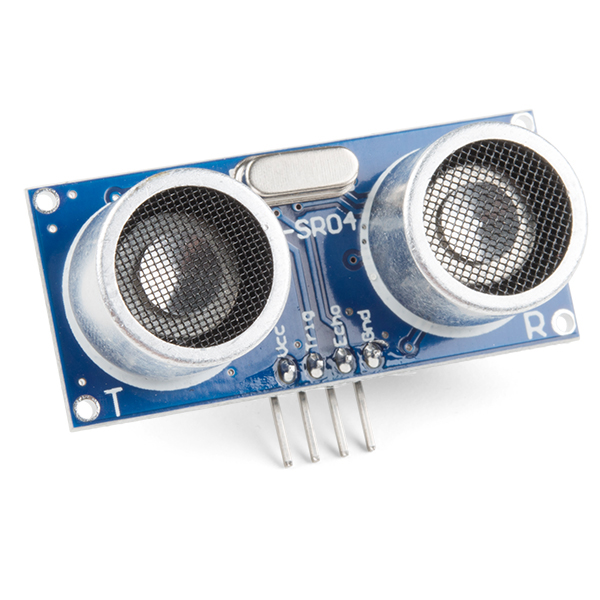
\includegraphics[width=1.75in]{ultrasonic.jpg} \\
            \caption{Ultrasonic Sensor (HC-SR04)}
            \label{fig:ultrasonic} % Optional: for referencing
        \end{figure}
    The HC-SR04 is a widely used ultrasonic sensor designed for distance measurement. It operates by emitting ultrasonic waves at a frequency of 40 kHz through its transmitter and receiving the echo reflected from an object via its receiver. The time taken for the echo to return is measured and used to calculate the distance to the object based on the speed of sound.
    
    \item \textbf{Microcontroller (NodeMCU/ESP8266)}\\
    \begin{figure}[H]
            \centering
            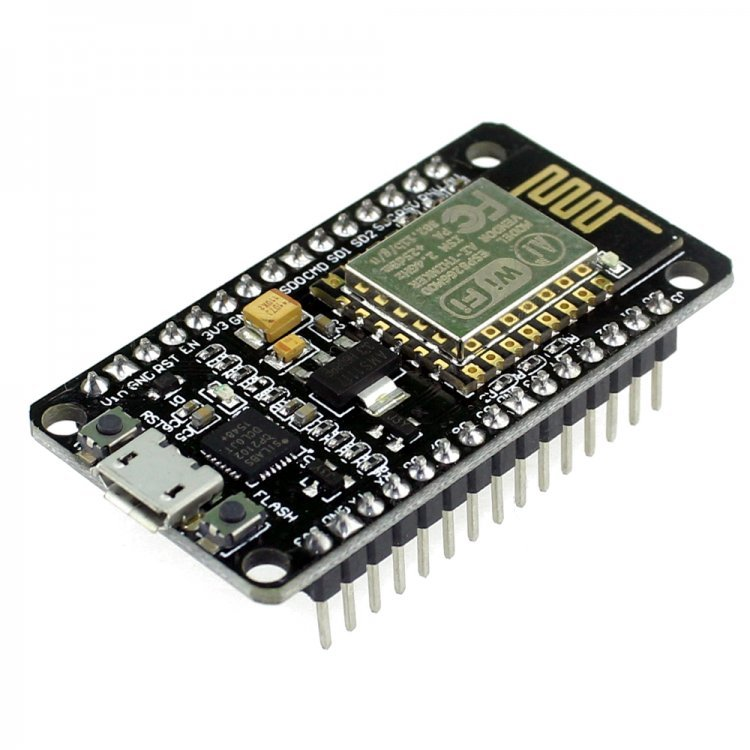
\includegraphics[width=1.75in]{esp.jpg} \\
            \caption{NodeMCU/ ESP8266}
            \label{fig:esp} % Optional: for referencing
        \end{figure}
    The ESP8266 is a low-cost Wi-Fi-enabled microcontroller that serves as the system's core processing unit. It processes data from sensors, executes control logic, and facilitates wireless communication with cloud platforms and mobile devices. Its built-in Wi-Fi module makes it ideal for IoT applications.

    
    \item \textbf{0.96'' OLED Display}\\
    \begin{figure}[H]
            \centering
            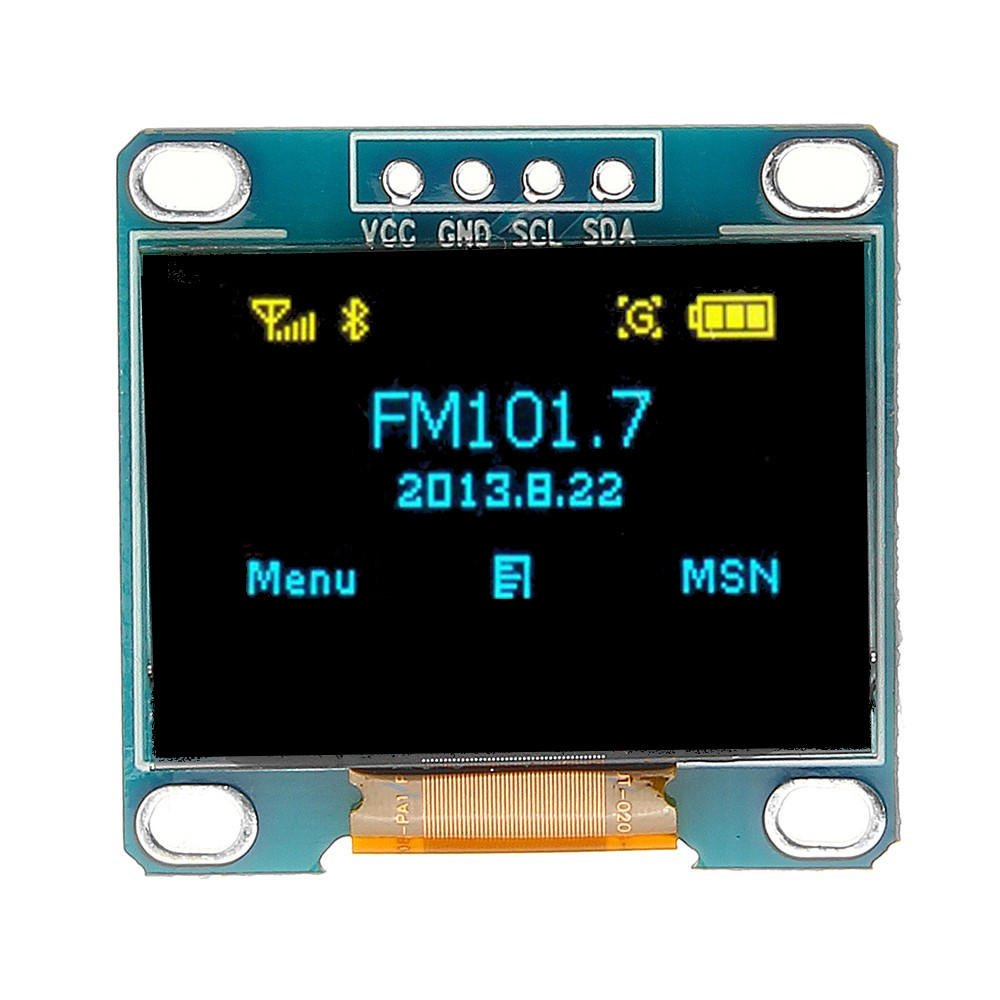
\includegraphics[width=1.75in]{oled.jpg} \\
            \caption{0.96''OLED Display}
            \label{fig:oled} % Optional: for referencing
        \end{figure}
    A 0.96-inch OLED display is a compact, high-contrast, and energy-efficient screen used in IoT projects to visually present data such as sensor readings, system status, or notifications.

    \item \textbf{Buzzer}\\
    \begin{figure}[H]
            \centering
            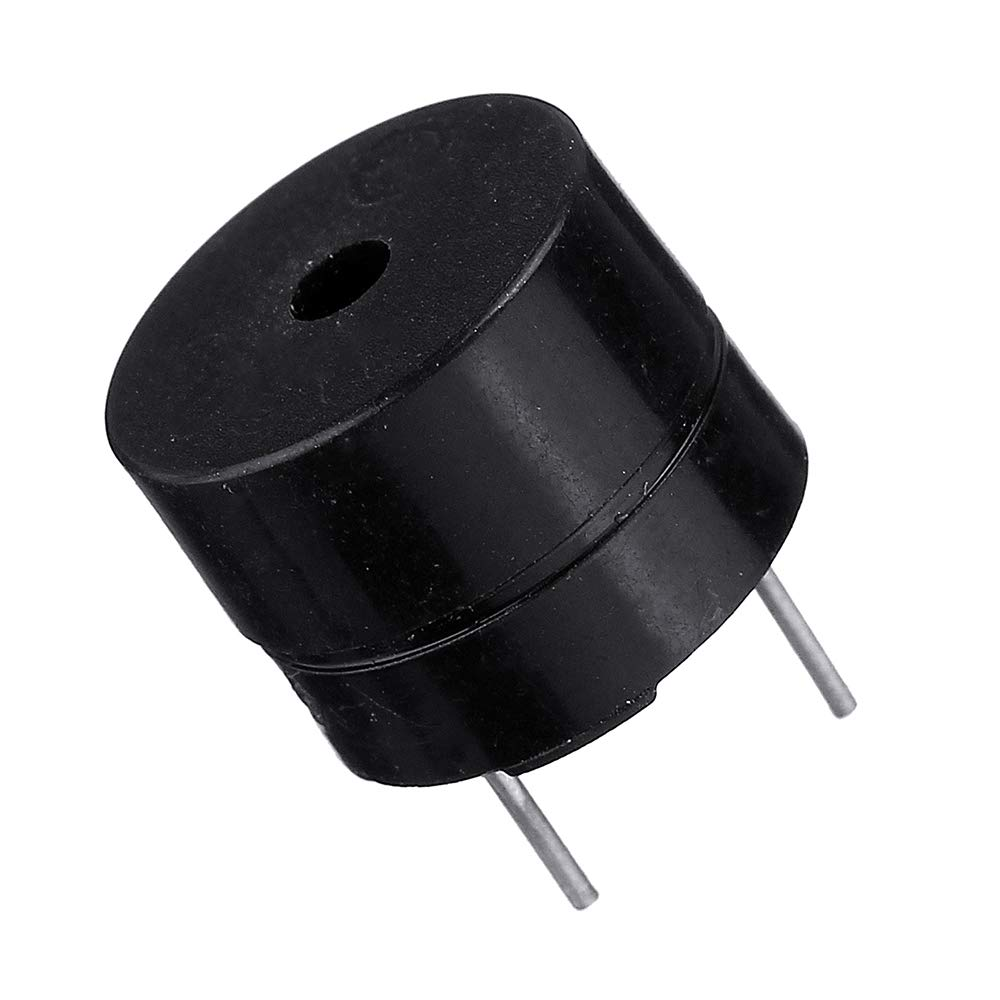
\includegraphics[width=1.75in]{buzzer.jpg} \\
            \caption{Buzzer}
            \label{fig:buzzer} % Optional: for referencing
        \end{figure}
    An electronic signaling device that produces sound. Commonly used in alarms, timers, and notifications in electronic circuits.
    
    \item \textbf{Push Buttons}\\
    \begin{figure}[H]
            \centering
            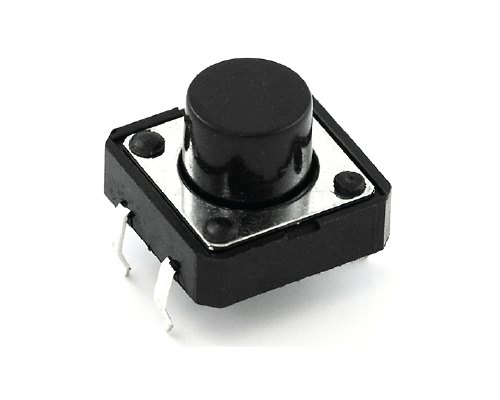
\includegraphics[width=1.75in]{push.png} \\
            \caption{Push Button}
            \label{fig:push-button} % Optional: for referencing
        \end{figure}
    Push button is a basic input device used in electronic and IoT projects to make or break a circuit connection when pressed. It has two terminals (pins) and functions as a single-pole, single-throw (SPST) switch, offering a simple way to send a digital signal to the microcontroller.
    
    \item \textbf{Jumper Wires}\\
    \begin{figure}[H]
            \centering
            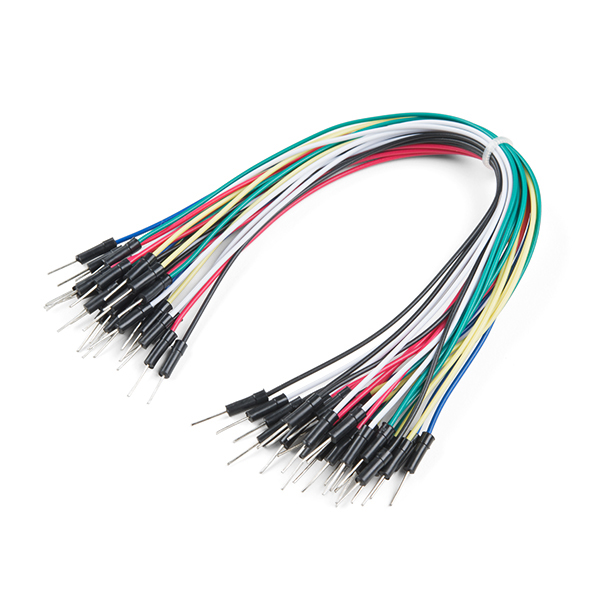
\includegraphics[width=1.75in]{jumper-wire.jpg} \\
            \caption{Jumper Wires}
            \label{fig:jumper-wire} 
        \end{figure}
    Short wires with connectors at each end, used to create temporary electrical connections on breadboards or between components. Facilitates quick and flexible connections in prototyping and troubleshooting electronic circuits.
    
    \item \textbf{AC to DC Converter (Relay)}\\
    \begin{figure}[H]
            \centering
            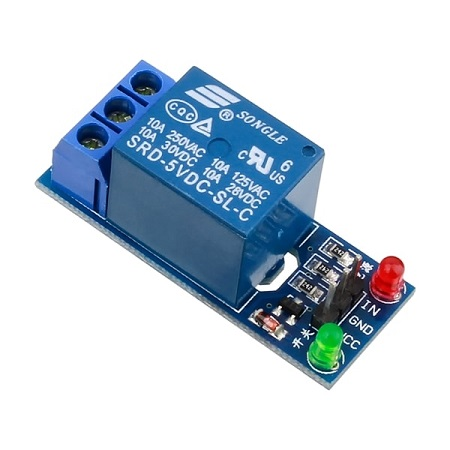
\includegraphics[width=1.75in]{relay.jpg} \\
            \caption{Single channel relay}
            \label{fig:relay} 
        \end{figure}
    Electromechanical switch used to control high-power devices with low-power signals. Enables the isolation between low-voltage circuits and high-voltage circuits, ensuring safety in control systems.
    
    \item \textbf{Breadboard}\\
    \begin{figure}[H]
            \centering
            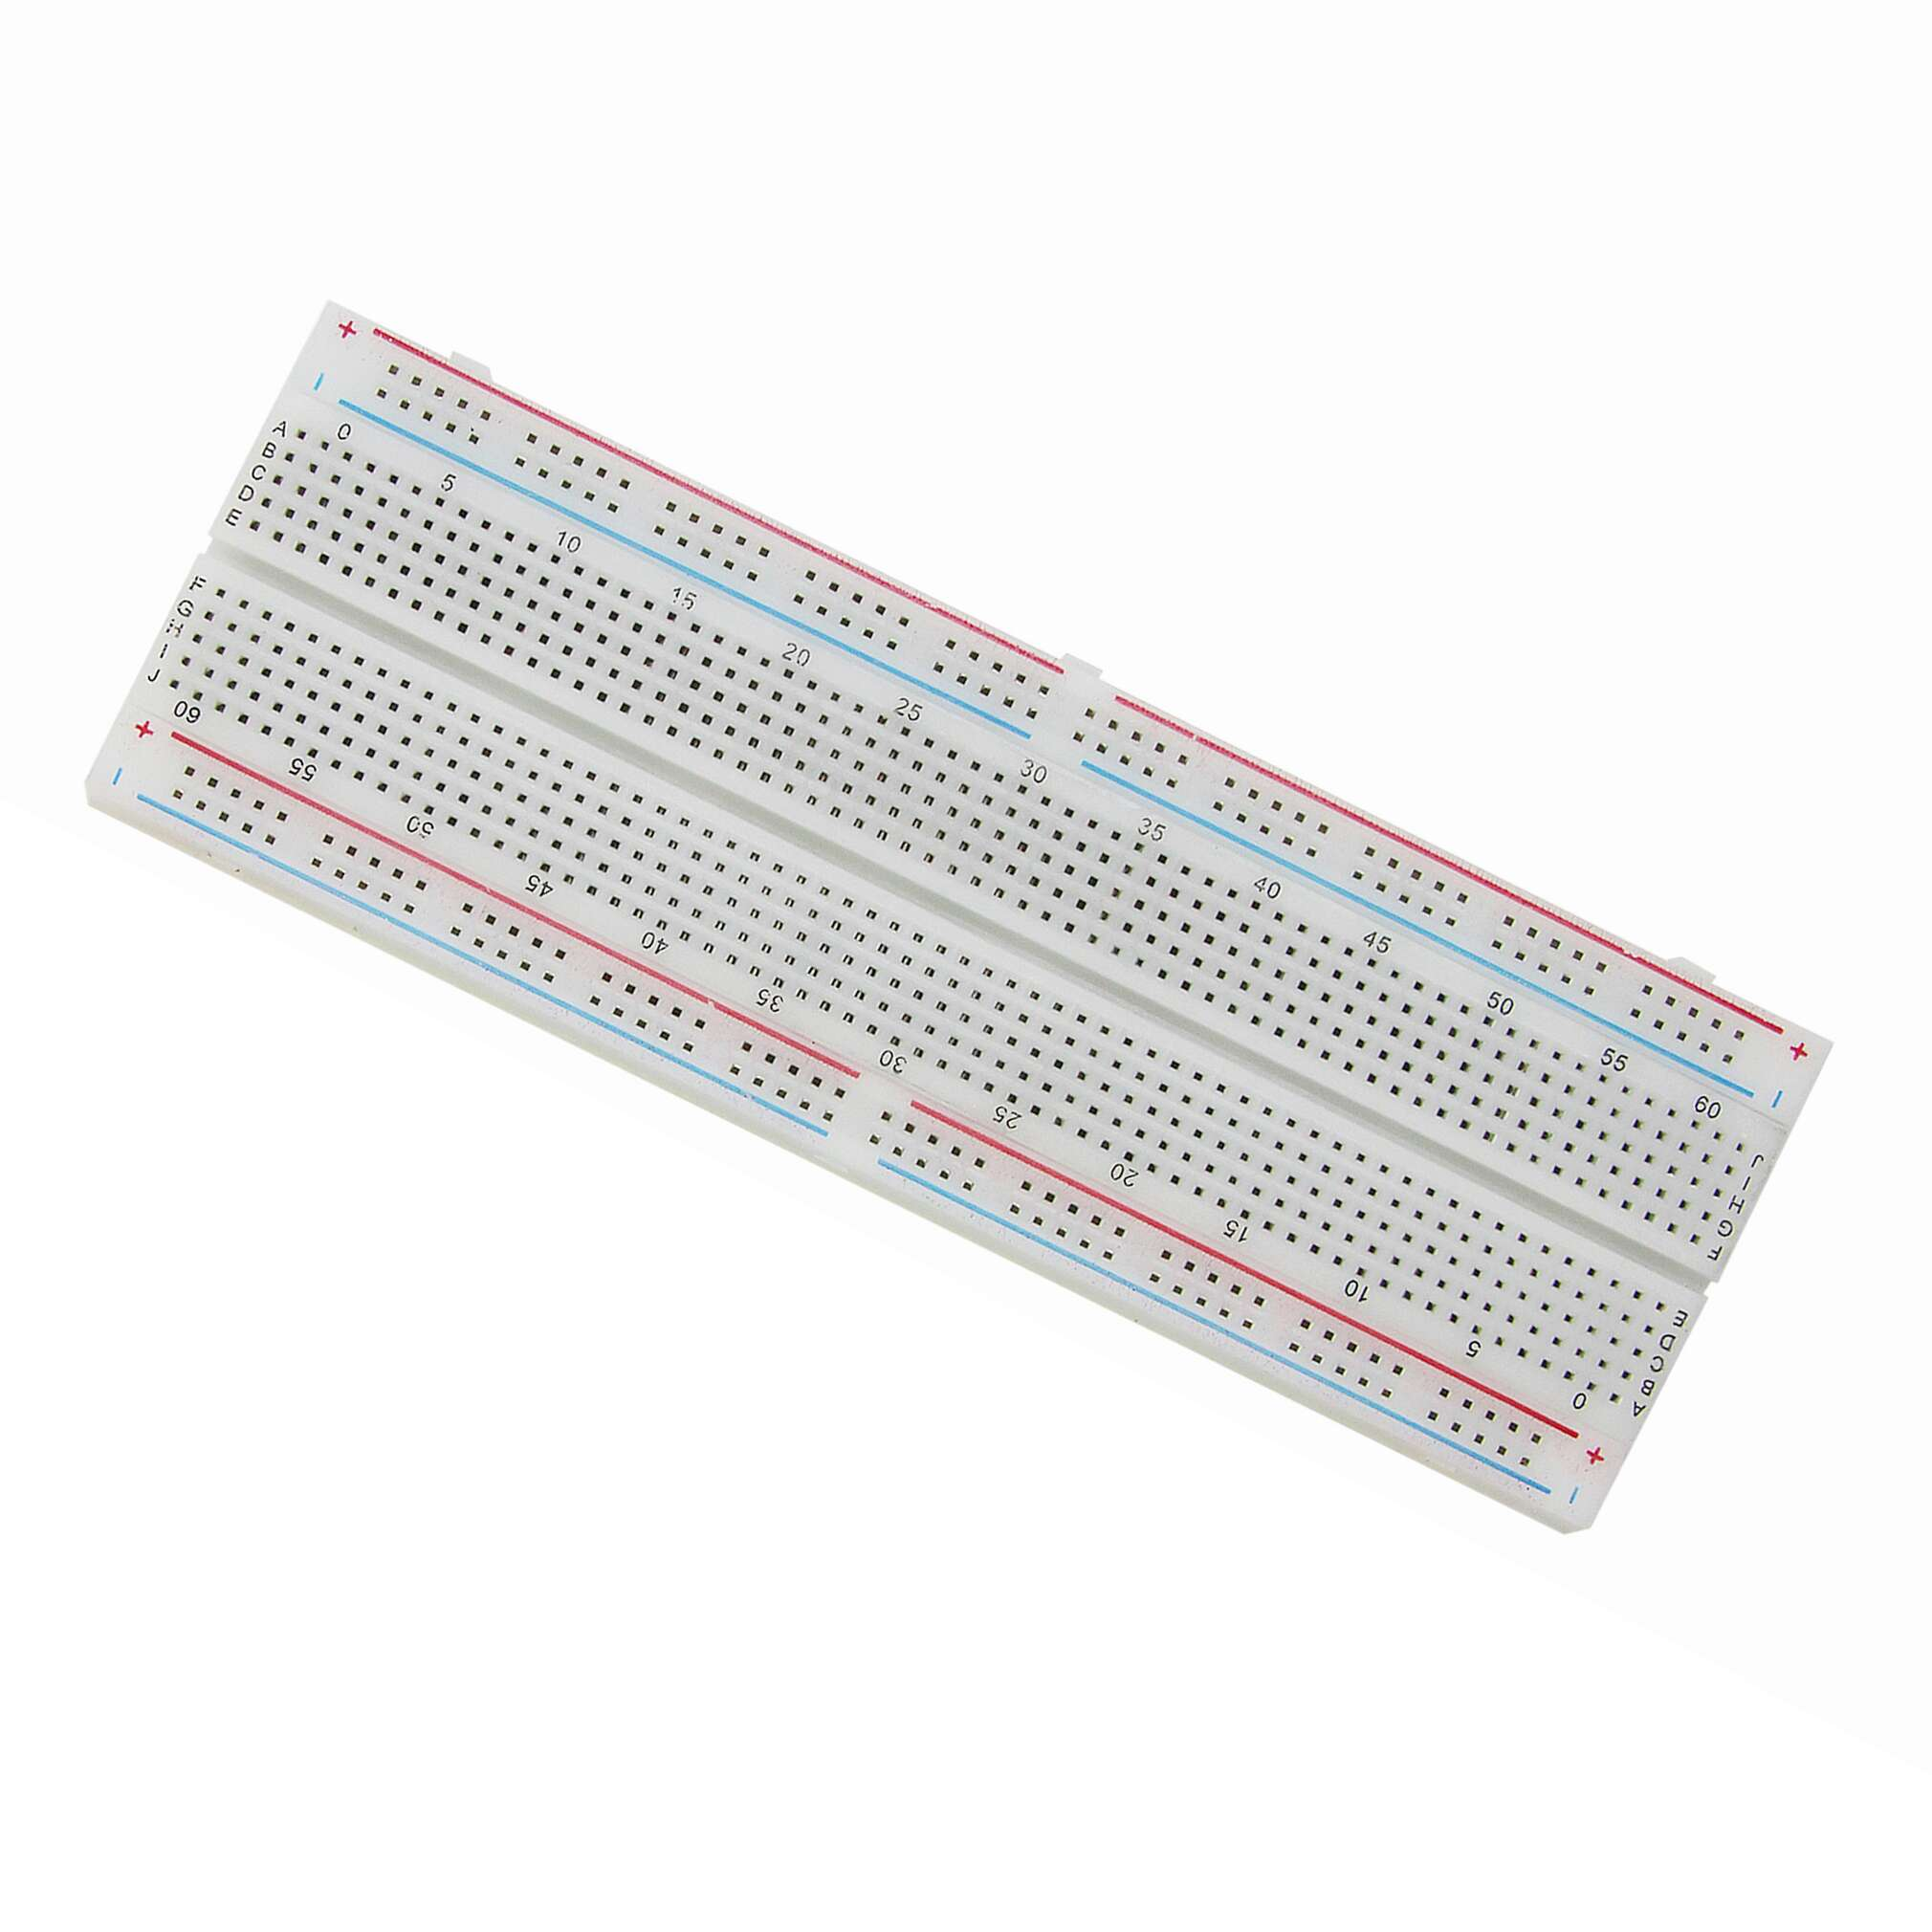
\includegraphics[width=1.75in]{breadboard.jpg} \\
            \caption{Breadboard}
            \label{fig:breadboard} 
        \end{figure}
    Prototyping tool for electronics projects, allowing components to be easily connected and tested without soldering. Ideal for rapid prototyping and experimenting with circuit designs.
    
    \item \textbf{Resistors}\\
    \begin{figure}[H]
            \centering
            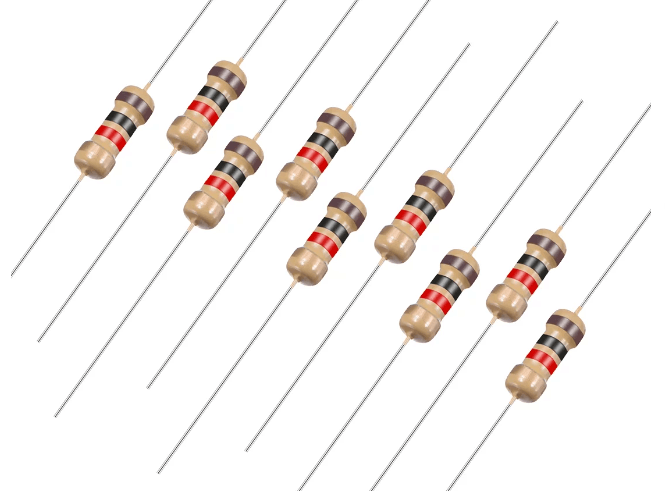
\includegraphics[width=1.75in]{resistors.png} \\
            \caption{Resistors}
            \label{fig:resistors} 
        \end{figure}
    A resistor is a passive electronic component used in IoT devices to limit current, divide voltages, or protect other components from excessive current flow. Resistors are critical for ensuring the safe and efficient operation of IoT circuits.
    
    \item \textbf{NPN Transistors}\\
    \begin{figure}[H]
            \centering
            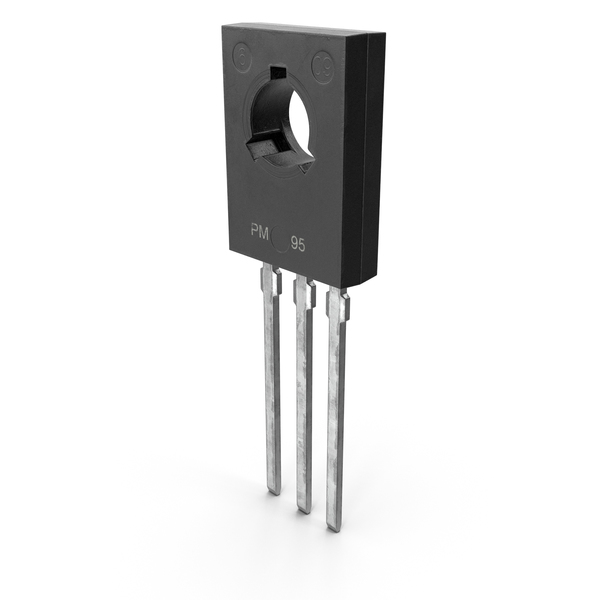
\includegraphics[width=1.75in]{transistors.jpg} \\
            \caption{NPN-Transistor}
            \label{fig:transistor} 
        \end{figure}
    An NPN transistor is commonly used as a switch or amplifier for controlling electronic signals in circuits. The NPN transistor consists of three layers of semiconductor material: n-type (negative), p-type (positive), and another n-type (negative), which are arranged as Emitter (E), Base (B), and Collector (C).
\end{enumerate}
    
    



\chapter{SYSTEM IMPLEMENTATION}
\section{Hardware Assembly and Circuit Diagram}
{\fontsize{12}{14}\selectfont
        \begin{figure}[H]
            \centering
            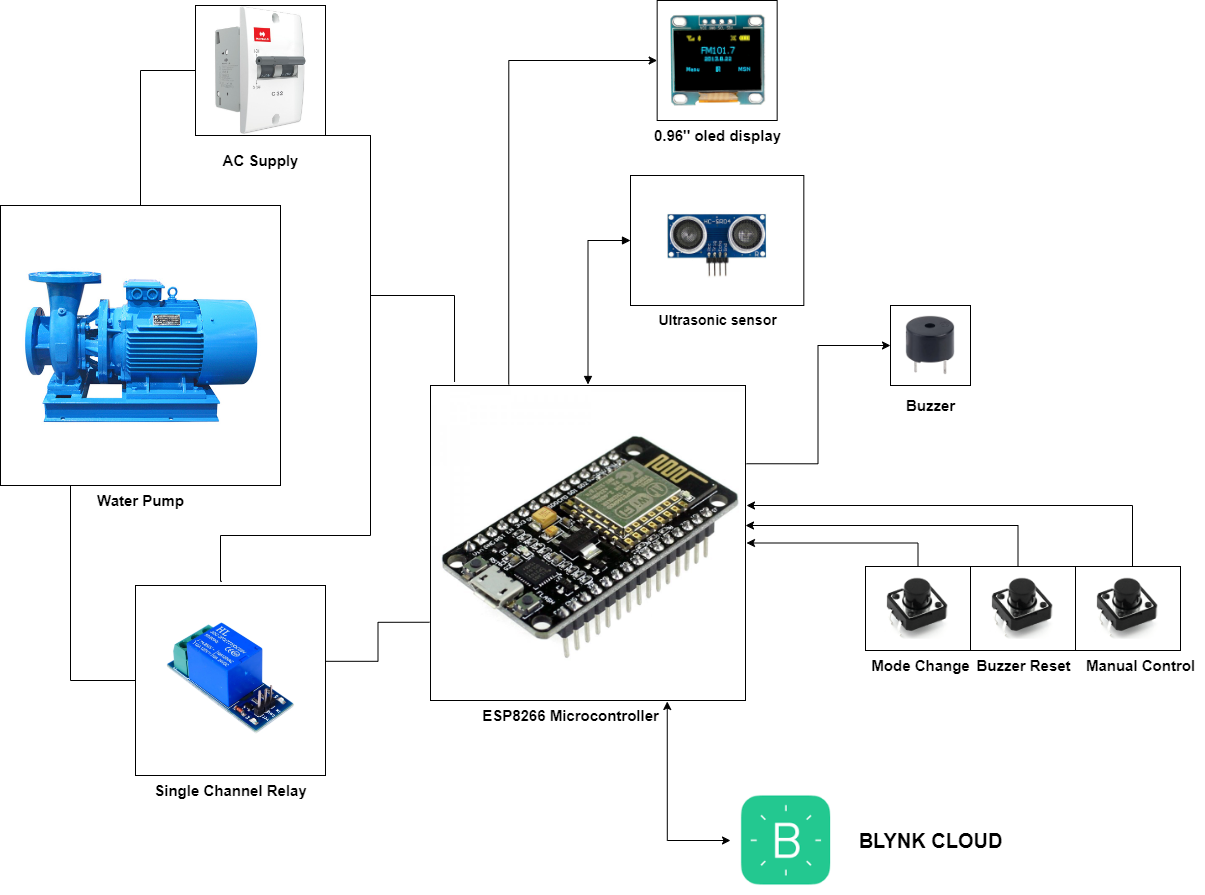
\includegraphics[width=6in]{diagram.png} \\
            \caption{Water Level Monitoring and Control Circuit Diagram}
            \label{fig:diagram} % Optional: for referencing
        \end{figure}

The hardware setup of this IoT-based water level monitoring and pump control system integrates multiple components to ensure real-time data acquisition, remote monitoring, and automated control of the water pump. \\
\newpage
\noindent
The following components are used in the system, with each playing a crucial role: \\
\begin{enumerate}
  \item \textbf{ESP8266 Microcontroller}\\
The ESP8266 is the core of the system, acting as the main controller for processing data from sensors, controlling output devices, and managing communication with the Blynk cloud platform. Its built-in Wi-Fi module allows seamless remote monitoring and control via the Blynk mobile application.

  \item \textbf{Ultrasonic Sensor (HC-SR04)}\\
The HC-SR04 ultrasonic sensor measures the distance between itself and the water surface, determining the water level in the tank. It sends high-frequency sound waves and calculates the time taken for the echo to return, which the ESP8266 processes to derive the water level.
  
  \item \textbf{0.96" OLED Display}\\
The OLED screen provides a local, real-time display of the water level. It serves as an immediate visual representation of the tank's status for users near the system.

  \item \textbf{Single Channel Relay Module}\\
The relay acts as a switch to control the water pump. Based on the water level thresholds processed by the ESP8266, the relay automatically activates or deactivates the water pump.

  \item \textbf{Water Pump}\\
The water pump fills the tank when the water level is low. Its operation is automated by the ESP8266 via the relay module.

  \item \textbf{Push Buttons}\\
    Three push buttons provide manual control and additional functionality:
    \begin{itemize}
      \item \textbf{Mode Change Button:} Toggles between different operational modes, such as automatic and manual control.
      \item \textbf{Buzzer Reset Button:} Silences the buzzer when a critical water level alert is triggered.
      \item \textbf{Manual Control Button:} Allows the user to turn the pump on or off manually.
    \end{itemize}

  \item \textbf{Buzzer}\\
The buzzer provides an audible alert for critical conditions, such as the tank being nearly empty or full. It ensures users are immediately aware of the system's status.

  \item \textbf{AC Power Supply}\\
The water pump is powered by an AC power supply, with the system ensuring safe and efficient operation.
\end{enumerate}

\noindent
\textbf{Circuit Diagram Explanation}\\
The circuit diagram visually represents the interconnections between the various hardware components. Each component is linked to the ESP8266, forming a centralized control system.
\noindent
The HC-SR04 ultrasonic sensor is connected to the ESP8266 via its trigger and echo pins. These signals are processed to determine the water level in the tank.
The OLED display communicates with the ESP8266 through an I2C interface to show real-time water level data.
The relay module connects to the ESP8266’s GPIO pins to control the water pump based on the processed data.
The push buttons are connected to the GPIO pins of the ESP8266, enabling manual user input for operational adjustments.
The buzzer is connected to another GPIO pin and is activated for critical alerts.
The ESP8266 sends data to the Blynk cloud platform via its Wi-Fi module, enabling remote monitoring and control through a smartphone app.
System Functionality
The ultrasonic sensor continuously monitors the water level and sends data to the ESP8266 for processing.
Based on predefined thresholds, the ESP8266 decides whether to turn the water pump on or off.
Data is displayed locally on the OLED screen and transmitted to the Blynk cloud for remote monitoring.
The push buttons allow users to override the system for manual control, reset alarms, or switch between modes.
Alerts are triggered via the buzzer and mobile notifications for low or critical water levels.
This circuit diagram reflects the modular and scalable nature of the system, making it suitable for future enhancements, such as additional sensors or water quality monitoring modules.

\section{Software Development and Integration with Arduino IDE and Blynk}
The software development process forms the backbone of the water monitoring and control system, enabling seamless communication between hardware components, real-time monitoring, and remote control functionality. The system leverages the Arduino IDE for microcontroller programming and the Blynk platform for IoT integration, creating a robust and user-friendly solution. This section provides a detailed explanation of the software design and implementation, highlighting its key components and functionalities.\\

\subsection{Arduino IDE Setup and Programming}
The Arduino IDE serves as the primary environment for programming the ESP8266 microcontroller. It provides tools for writing, debugging, and uploading code, ensuring efficient interaction with the system's hardware components.
\begin{enumerate}
  \item \textbf{Environment Setup:}\\
    \begin{itemize}
      \item The Arduino IDE is configured to support the ESP8266 microcontroller by adding the ESP8266 board manager through the IDE preferences. This allows seamless compatibility between the IDE and the hardware.
      \item Relevant drivers are installed to ensure the microcontroller is recognized by the computer.
    \end{itemize}
  \item \textbf{Library Installation:}
    \begin{itemize}
      \item Essential libraries are integrated into the IDE to enable specific functionalities:
      \begin{itemize}
        \item Blynk Library: Facilitates communication between the ESP8266 and the Blynk cloud platform.
        \item Adafruit GFX and SSD1306 Libraries: Support the OLED display module for real-time data visualization.
        \item Ultrasonic Sensor Library: Simplifies the interaction with the HC-SR04 ultrasonic sensor.
      \end{itemize}
      \item These libraries are added through the library manager or manually imported into the project.
    \end{itemize}
  \item \textbf{Code Development:}
    The software is designed to handle multiple tasks simultaneously, ensuring the system operates efficiently. Key code components include:
    \begin{itemize}
      \item \textbf{Sensor Data Acquisition:}\\
        The HC-SR04 ultrasonic sensor measures the water level by calculating the distance between the sensor and the water surface. The sensor's echo and trigger pins are defined, and the data is read using precise timing functions.
      \item \textbf{Data Processing:}\\
        The raw sensor data is processed into meaningful water level values, which are then used to determine system actions. For instance, threshold levels are set to activate or deactivate the water pump.
      \item \textbf{OLED Display Control:}\\
        The processed water level data is sent to the OLED display for local visualization. The display updates in real-time to provide an intuitive interface for users.
    
      \item \textbf{Buzzer Alerts:}\\
        The buzzer is activated when critical water levels are reached, providing an audible alert to ensure timely action.
    
      \item \textbf{Automation Logic:}\\
        Control logic is implemented to automatically switch the water pump on or off based on water level thresholds. This reduces the need for manual intervention.
    \end{itemize}
    \item \textbf{Testing and Debugging:}
    The Arduino IDE’s serial monitor is utilized extensively during development to monitor real-time data from the microcontroller. Debugging tools within the IDE help identify and resolve any issues in the code, ensuring smooth operation.
\end{enumerate}

\subsection{Blynk Cloud Integration}
Blynk is employed as the IoT platform to enable real-time monitoring and remote control through a mobile application. It acts as a bridge between the ESP8266 microcontroller and the user, providing an intuitive interface for system management.
\begin{enumerate}
  \item \textbf{Cloud Platform Configuration:}\\
    A Blynk account is created, and a new project is set up within the mobile application.
    An authentication token generated by Blynk is included in the Arduino code, linking the microcontroller to the cloud platform.
  \item \textbf{Wi-Fi Connectivity:}\\
    The ESP8266 is programmed to connect to a Wi-Fi network using the SSID and password provided in the code. This connection enables the microcontroller to send and receive data via the Blynk cloud.
  \item \textbf{Mobile Application Widgets:}\\
    The Blynk mobile application is configured with various widgets to enhance user interaction:
    \begin{itemize}
      \item Value Display: Displays the current water level in real-time.
      \item Button Widget: Allows manual control of the water pump.
      \item Gauge Widget: Provides a graphical representation of the water level.
      \item Notification Widget: Sends alerts to the user’s mobile device for critical events, such as low or high water levels.
    \end{itemize}
  \item \textbf{Data Transmission:}
    \begin{itemize}
      \item The processed water level data from the ultrasonic sensor is transmitted to the Blynk cloud via virtual pins.
      \item The Blynk platform relays this data to the mobile application, where users can monitor it in real-time.
    \end{itemize}
  \item \textbf{Control Mechanisms:}
    \begin{itemize}
      \item Users can control the water pump remotely through the Blynk app.
      \item Manual overrides are supported, allowing users to activate or deactivate the pump as needed, irrespective of the automation logic.
    \end{itemize}
  \item \textbf{Automation Features:}\\
    The Blynk platform integrates seamlessly with the automation logic in the Arduino code. For example, when a critical water level is reached, the system sends a notification to the user while simultaneously triggering the appropriate system response.
\end{enumerate}

\noindent
By combining Arduino IDE and Blynk, the system benefits from a simple yet powerful development and integration process. The Arduino IDE provides flexibility and control over the microcontroller, while Blynk offers user-friendly tools for IoT integration. Together, they create a system that is reliable, responsive, and accessible.\\
\noindent
This software setup allows for real-time monitoring, efficient automation, and intuitive remote control, making it a vital component of the water monitoring and control system.
}
    

\chapter{CONCLUSION}
\section{Summary of the Project}
{
\fontsize{12}{14}\selectfont
\noindent
    The Smart Water Level Monitoring System using a microcontroller successfully achieved its objectives of monitoring and managing water levels in real-time. The system efficiently utilizes ultrasonic sensors to measure the water level, calculates the percentage of tank capacity, and provides clear visual feedback via an OLED display and the Blynk platform. Additionally, the system includes a buzzer alert to notify users when the tank is almost full, preventing water wastage due to overflow. This solution demonstrates the potential of integrating IoT and embedded systems to automate and improve water management in households, industries, and agriculture. The project is a cost-effective, user-friendly, and reliable solution for addressing water monitoring challenges.
} 

\vspace{0.2cm}
\section{Recommendation for Future Research}
\fontsize{12}{14}\selectfont{
\begin{enumerate}
    \item \textbf{Integration with Automated Pump Systems} \\
    Future iterations of the Smart Water Level Monitoring System could incorporate an automated pump control mechanism to enhance its functionality and user convenience. By integrating a relay module or a similar device, the system could automatically start or stop the water pump based on predefined water levels, eliminating the need for manual intervention. For instance, the pump could automatically turn on when the water level falls below a certain threshold and turn off when the tank is almost full. This automation not only reduces the risk of overflow or dry runs but also improves energy efficiency and water resource management. Furthermore, such an enhancement would be especially beneficial for households, industries, and agricultural setups where timely water replenishment is critical.

    \item \textbf{Ultrasonic Waterproof Sensors} \\
    The integration of ultrasonic waterproof sensors, such as the widely used JSN-SR04T, can significantly enhance the accuracy and reliability of the water level monitoring system. These sensors operate by emitting ultrasonic sound waves and measuring the time taken for the waves to return after bouncing off the water's surface. This non-contact method ensures precise measurements without any wear and tear caused by direct exposure to water. Additionally, their waterproof design allows them to function effectively in submerged or high-humidity environments, making them ideal for water tanks, reservoirs, and other applications. The JSN-SR04T, in particular, is known for its durability, affordability, and resistance to harsh environmental conditions, ensuring long-term reliability and low maintenance. Adopting such sensors ensures that the system remains robust and accurate, even under challenging operational conditions.

    \item \textbf{Solar Power Integration} \\
    Integrating solar power into the water level monitoring system offers a sustainable and energy-efficient solution, especially for remote areas with limited or unreliable electricity access. Solar panels can provide the necessary energy to power the sensors, microcontroller, and additional components, making the system self-sufficient and reducing dependency on external power sources. This approach not only lowers operational costs but also aligns with environmental sustainability goals by utilizing renewable energy. In addition, a battery backup can be added to store excess solar energy, ensuring uninterrupted operation during nighttime or cloudy weather. The adoption of solar power not only broadens the applicability of the system but also enhances its resilience in diverse environments, including rural and off-grid areas.

    \item \textbf{Support for Multiple Tanks} \\
    To increase the versatility and scalability of the water level monitoring system, future upgrades could include the ability to monitor multiple tanks simultaneously. This feature would be particularly useful for large-scale applications, such as in residential complexes, industrial plants, or agricultural irrigation systems, where multiple water storage units are used. By incorporating multiple sensor inputs and designing a centralized control interface, users could monitor and manage the water levels of all tanks from a single platform, such as the Blynk app or a web dashboard. Additionally, the system could incorporate separate alerts and automated controls for each tank, further streamlining water management. Such a multi-tank monitoring system would provide a comprehensive solution for efficient water usage and conservation across different sectors.

    \item \textbf{Leakage Detection} \\
    Adding a leakage detection feature to the water level monitoring system would provide an additional layer of functionality and ensure better water conservation. This could be achieved by integrating flow sensors or pressure transducers capable of detecting abnormal flow rates or pressure drops, which are indicative of leaks. When a potential leakage is identified, the system could send real-time alerts to the user via the Blynk platform or trigger an automatic shutoff mechanism to prevent water wastage. Such a feature would be invaluable in both residential and industrial setups, where undetected leaks could lead to significant water loss and increased utility costs. By implementing this upgrade, the system would not only monitor water levels but also actively contribute to minimizing water wastage, aligning with global efforts toward sustainable water resource management.
\end{enumerate}
}


\chapter*{REFERENCES}
\addcontentsline{toc}{chapter}{REFERENCES}
\begin{enumerate}
  \item Arduino Documentation, \\
  \textcolor{blue}\faLink \hspace{0.1cm} \href{https://docs.arduino.cc/}{\textcolor{blue}{https://docs.arduino.cc/}}
  
  \item Blynk Documentation \\
  \textcolor{blue}\faLink \hspace{0.1cm} \href{https://docs.blynk.io/en}{\textcolor{blue}{https://docs.blynk.io/en}}
  
  \item Wireless Communications With RF-Based Energy Harvesting: From Information Theory to Green Systems, \textit{IEEE Xplore}, \\
  \textcolor{blue}\faLink \hspace{0.1cm} \href{https://ieeexplore.ieee.org/document/8125666}{\textcolor{blue}{https://ieeexplore.ieee.org/document/}}
  
  \item Smart Water Level Monitoring System Using Internet of Things (IoT), \textit{ResearchGate},  \\
  \textcolor{blue}\faLink \hspace{0.1cm} \href{https://www.researchgate.net/publication/369408401_Smart_Water_Level_Monitoring_System_Using_Internet_of_Things_IoT}{\textcolor{blue}{https://www.researchgate.net/publication/}}
\end{enumerate}






\chapter*{APPENDICES}
\addcontentsline{toc}{chapter}{APPENDICES}
\section*{APPENDIX A : Source Code}
        
\begin{lstlisting}[language=C]    
#define BLYNK_TEMPLATE_ID "TMPL3IB6tWBiU"
#define BLYNK_TEMPLATE_NAME "Esp8266 Water Level"
#define BLYNK_AUTH_TOKEN "4fqrL-V4lYbfVKfVsgYarGmM0JtSCkmy"

// Your WiFi credentials
char ssid[] = "Your_WiFi_Network";   // WiFi Name
char pass[] = "Your_password";        // WiFi Password

#include <BlynkSimpleEsp8266.h>
#include <SPI.h>
#include <Wire.h>
#include <Adafruit_GFX.h>
#include <Adafruit_SH110X.h>
#define BLYNK_PRINT Serial
#include <ESP8266WiFi.h>

// Define pins for ESP8266
#define D4 2   // GPIO2
#define D5 14  // GPIO14
#define D6 12  // GPIO12

#define i2c_Address 0x3c // Initialize with the I2C addr 0x3C
#define SCREEN_WIDTH 128 // OLED display width, in pixels
#define SCREEN_HEIGHT 64 // OLED display height, in pixels
#define OLED_RESET -1    // QT-PY / XIAO

Adafruit_SH1106G display = Adafruit_SH1106G(SCREEN_WIDTH, SCREEN_HEIGHT, &Wire, OLED_RESET);

const int trigPin = D5;
const int echoPin = D6;
const int buzzer = D4;

const float tankHeight = 15; // Height of the water tank in cm

float duration, distance, waterLevel;

bool buzzerEnabled = true; // Flag to enable/disable the buzzer

// Timer for sending data to Blynk
BlynkTimer timer;

void setup() {
  // Debug console
  Serial.begin(9600);

  // Blynk setup
  Blynk.begin(BLYNK_AUTH_TOKEN, ssid, pass);

  // Ultrasonic sensor
  pinMode(trigPin, OUTPUT);
  pinMode(echoPin, INPUT);
  pinMode(buzzer, OUTPUT);

  // OLED setup
  delay(250); // Wait for the OLED to power up
  display.begin(i2c_Address, true);
  display.display(); // Show Adafruit splash screen
  display.clearDisplay();

  // Timer to send data to Blynk
  timer.setInterval(1000L, sendToBlynk); // Send data every second
}

void loop() {
  Blynk.run();  // Run Blynk
  timer.run();  // Run the timer

  // Measure distance
  digitalWrite(trigPin, LOW);
  delayMicroseconds(2);
  digitalWrite(trigPin, HIGH);
  delayMicroseconds(10);
  digitalWrite(trigPin, LOW);

  duration = pulseIn(echoPin, HIGH);
  distance = (duration * 0.0343) / 2;

  // Calculate water level
  waterLevel = ((tankHeight - distance) / tankHeight) * 100;
  waterLevel = constrain(waterLevel, 0, 100); // Constrain value to 0-100%

  // Display water level on OLED
  String levelStr = "Water Level: " + String(waterLevel, 1) + "%";
  displayText(levelStr.c_str(), 0, 2, 2);

  // Buzzer logic
  if (buzzerEnabled && distance <= 5) {
    tone(buzzer, 1000);  // Sound buzzer at 1kHz
  } else {
    noTone(buzzer);      // Turn off the buzzer
  }

  delay(500); // Update every half second
}

/**
 * Function to send data to Blynk
 */
void sendToBlynk() {
  Blynk.virtualWrite(V1, waterLevel); // Send water level percentage to Virtual Pin V1
  Blynk.virtualWrite(V2, distance);  // Send distance to Virtual Pin V2 (optional)
}

/**
 * Function to display text on the OLED screen
 * @param text The string to display
 * @param x The x-coordinate for the starting position
 * @param y The y-coordinate for the starting position
 * @param textSize The size of the text (1 = small, 2 = medium, etc.)
 */
void displayText(const char *text, int x, int y, int textSize) {
  display.clearDisplay();            // Clear the display buffer
  display.setTextSize(textSize);     // Set the text size
  display.setTextColor(SH110X_WHITE); // Set text color
  display.setCursor(x, y);           // Set cursor position
  display.println(text);             // Print the text
  display.display();                 // Display the updated buffer
}

/**
 * Function to handle Blynk virtual pin V5 for enabling/disabling the buzzer
 */
BLYNK_WRITE(V5) {
  int value = param.asInt(); // Get the value from the Blynk app (0 or 1)
  buzzerEnabled = (value == 1); // Enable buzzer if 1, disable if 0
  Serial.print("Buzzer Enabled: ");
  Serial.println(buzzerEnabled ? "Yes" : "No");
}

\end{lstlisting}


\newpage
\section*{APPENDIX B : Calibration and Setup Guide}
\vspace*{0.6cm}
{\fontsize{12}{14}\selectfont{

    \begin{enumerate}
    \item \textbf{Hardware Setup:}
    \begin{itemize}
        \item \textbf{Components Required:}
        \begin{itemize}
            \item ESP8266 (e.g., NodeMCU)
            \item Ultrasonic sensor (HC-SR04)
            \item OLED display (SH1106)
            \item Buzzer
            \item Jumper wires
            \item Power supply (USB or battery)
            \item Water tank for testing
        \end{itemize}
        \item \textbf{Connections:}
        \begin{itemize}
            \item \textbf{Ultrasonic Sensor (HC-SR04):}
            \begin{itemize}
                \item Trig pin $\rightarrow$ GPIO14 (D5)
                \item Echo pin $\rightarrow$ GPIO12 (D6)
                \item VCC $\rightarrow$ 5V
                \item GND $\rightarrow$ GND
            \end{itemize}
            \item \textbf{OLED Display (SH1106):}
            \begin{itemize}
                \item SDA $\rightarrow$ D2 (I2C Data)
                \item SCL $\rightarrow$ D1 (I2C Clock)
                \item VCC $\rightarrow$ 3.3V
                \item GND $\rightarrow$ GND
            \end{itemize}
            \item \textbf{Buzzer:}
            \begin{itemize}
                \item Positive terminal $\rightarrow$ GPIO2 (D4)
                \item Negative terminal $\rightarrow$ GND
            \end{itemize}
        \end{itemize}
        \item \textbf{Powering the Circuit:}
        \begin{itemize}
            \item Ensure the ESP8266 is powered via USB or a 3.3V battery source.
            \item Verify all connections before powering on.
        \end{itemize}
    \end{itemize}
    
    \item \textbf{Software Configuration:}
    \begin{itemize}
        \item Install Arduino IDE:
        \begin{itemize}
            \item Download and install the Arduino IDE from \url{https://www.arduino.cc/}.
        \end{itemize}
        \item Install Necessary Libraries:
        \begin{enumerate}
            \item Open the Arduino IDE.
            \item Navigate to \textbf{Sketch > Include Library > Manage Libraries}.
            \item Search for and install:
            \begin{itemize}
                \item \texttt{Blynk}
                \item \texttt{Adafruit GFX Library}
                \item \texttt{Adafruit SH110X}
            \end{itemize}
        \end{enumerate}
        \item Set Up Blynk:
        \begin{enumerate}
            \item Create a new project in the Blynk app.
            \item Select the device as \textbf{ESP8266} and connection type as \textbf{WiFi}.
            \item Note the Auth Token provided and replace it in the code.
        \end{enumerate}
        \item Configure WiFi Credentials:
        \begin{itemize}
            \item Replace the placeholders for SSID and password in the code:
            \begin{verbatim}
            char ssid[] = "YourWiFiName";
            char pass[] = "YourWiFiPassword";
            \end{verbatim}
        \end{itemize}
        \item Upload the Code:
        \begin{enumerate}
            \item Select the board as \textbf{NodeMCU 1.0} in \textbf{Tools > Board}.
            \item Select the correct COM port.
            \item Click on the upload button to flash the code onto the ESP8266.
        \end{enumerate}
    \end{itemize}
    
    \item \textbf{Calibration:}
    \begin{itemize}
        \item Tank Height:
        \begin{itemize}
            \item Measure the height of the water tank in centimeters.
            \item Replace the value of \texttt{tankHeight} in the code with the measured height.
        \end{itemize}
        \item Testing the Ultrasonic Sensor:
        \begin{itemize}
            \item Position the sensor at the top of the water tank.
            \item Measure the distance manually using a ruler and compare it with the sensor's output.
            \item Adjust placement for accurate readings.
        \end{itemize}
    \end{itemize}
    
    \item \textbf{Testing and Validation:}
    \begin{itemize}
        \item OLED Display:
        \begin{itemize}
            \item Ensure the display shows the water level in percentage.
            \item Adjust the screen connections if it remains blank.
        \end{itemize}
        \item Buzzer:
        \begin{itemize}
            \item Test the buzzer functionality by lowering the water level to trigger the threshold (\texttt{distance <= 5 cm}).
            \item Enable/disable the buzzer via the Blynk app by toggling Virtual Pin V5.
        \end{itemize}
        \item Blynk Dashboard:
        \begin{itemize}
            \item Add widgets in the Blynk app:
            \begin{itemize}
                \item Label for Virtual Pin V1 (Water Level Percentage).
                \item Label for Virtual Pin V2 (Distance in cm).
                \item Button for Virtual Pin V5 (Buzzer control).
            \end{itemize}
            \item Validate data updates in real-time.
        \end{itemize}
    \end{itemize}
    
    \item \textbf{Troubleshooting:}
    \begin{itemize}
        \item No Display on OLED:
        \begin{itemize}
            \item Verify the I2C address (\texttt{0x3c}) and connections.
            \item Ensure the \texttt{Adafruit\_SH1106} library is properly installed.
        \end{itemize}
        \item Buzzer Not Working:
        \begin{itemize}
            \item Check GPIO2 (\texttt{D4}) connections.
            \item Ensure \texttt{buzzerEnabled} is set to \texttt{true}.
        \end{itemize}
        \item Blynk Not Connecting:
        \begin{itemize}
            \item Confirm WiFi credentials and internet connectivity.
            \item Check the Auth Token in the code.
        \end{itemize}
        \item Ultrasonic Sensor Issues:
        \begin{itemize}
            \item Test the sensor separately using a simple distance measurement script.
            \item Ensure clean and unobstructed sensor placement.
        \end{itemize}
    \end{itemize}
\end{enumerate}

} 


\end{document}
